\subsection{Data Set Analysis via Dimensionality Reduction with Neural Networks - Information Landscapes}

When analyzing data sets for qualities such as diversity, it is important to make the distance measure consistent with the predictive model.  For example, if the prediction were made with a Gaussian process, it would be wise to use the distance model built into the kernel to analyze the diversity of the datasets studied.  This becomes somewhat more complex when the predictive method does not have a well defined distance measure built into it, such as a neural network.  Simply analyzing the diversity of the inputs through the use of a Tanimoto distance histogram, for example, is potentially a dangerous path since it does not acknowledge the highly connected nature of the neurons in a neural network.  We instead utilize an alternative measure, in which a neural network itself is used to compress the data into a resonable number of dimensions,~\cite{hinton_reducing_2006} upon which a visual inspection can reveal the diversity of the dataset.

This is achieved through training an unsupervised neural network, of which the loss function of each layer is determined by how well the output matches that of the previous layer.  Through sequential reduction in the number of neurons, the principle components of an input signal are amplified, and can be sampled.  To fine tune the weights of this neural network, the funneling architecture is mirrored, and the weights adjusted so that a loss function comparing the input and output of the network is minimized.

\begin{figure}[h!]
\centering
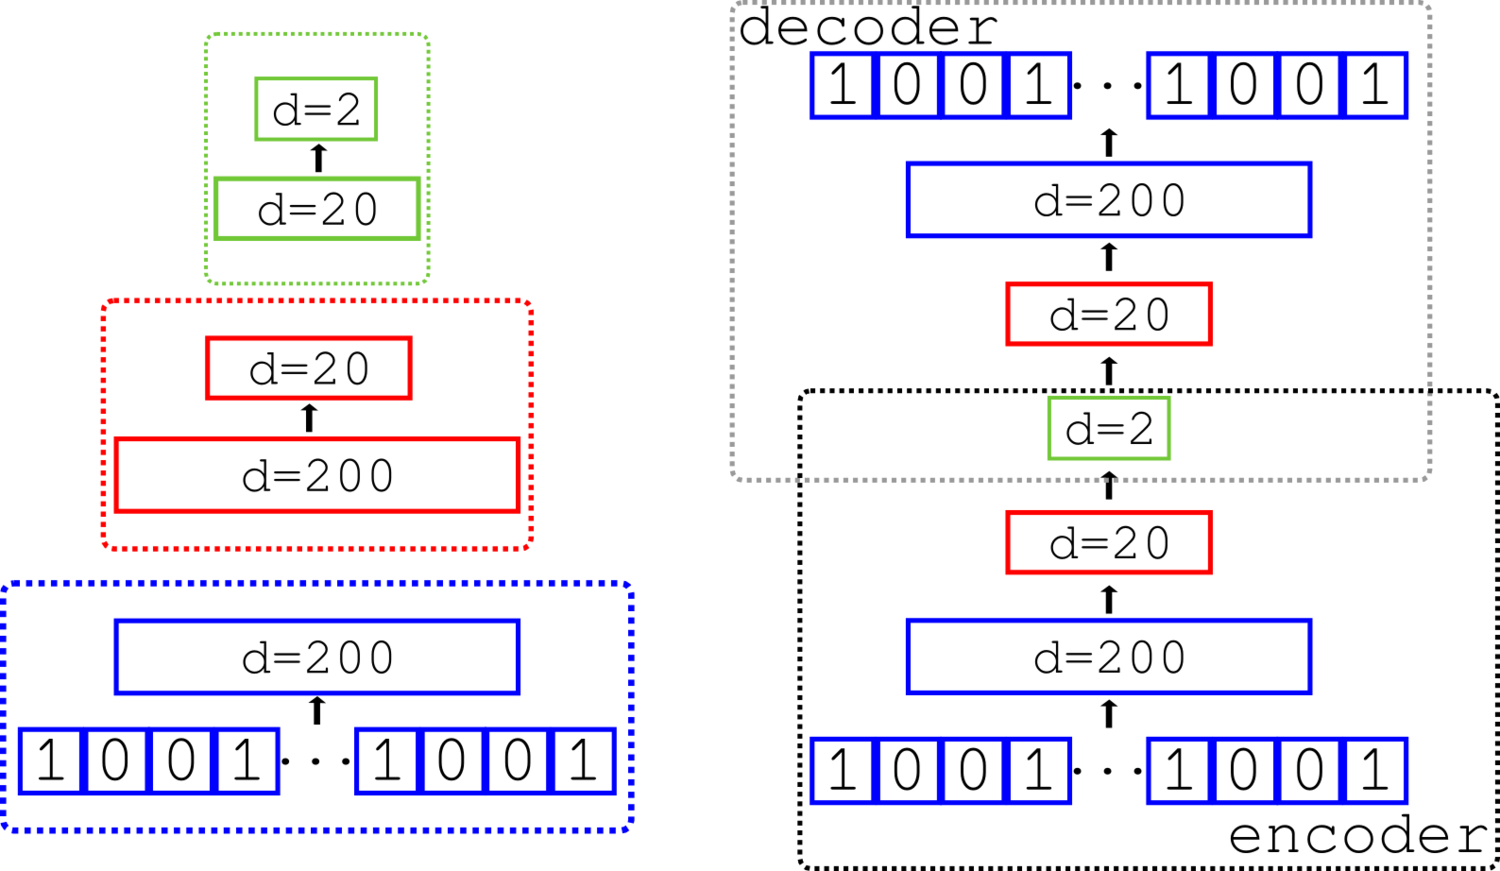
\includegraphics[width=1\columnwidth]{figures/nnet_decomp.png}
\caption{Neural networks can be used to compress data into a few, representative directions. In order to properly condition the weights of the neural network to be close to an optimal solution, the weights of each layer are pre-trained so that the layer reproduces the output of the previous layer (left).  These layers are then stacked into a funnel first decreasing in size (the encoder) and then increasing in size (the decoder).  Finally, the weights are fine-tuned to minimize reconstruction error (right).}
\label{fig:nn_decomp}
\end{figure}

The distributions of these network derived principle components were further investigated through the calculation of pairwise component distances. These distances were normalized so that the maximum distance was set at 1.0, and the minimum set to be 0.0. It can be seen from Figure \ref{fig:dist_hists}, that all of the sets are reasonably diverse in the eyes of the neural network.  As seen from figure 3, these sets are reasonably diverse in the eyes of the neural network. This statement may be counterintuitive from the chemical perspective, as perhaps one can think that molecules to carry out a specific task are likely to be more chemically similar. Global diversity measures can often give a misleading view into how models work on data. These measures can be thought of as a map of the local surroundings in chemical space.  To extend the metaphor, if you are looking to find the best place for a picnic, it is more helpful to have a streetmap than a globe.